% cg-layout: pipeline
% figure check fixture (#1064): an era's title wider than its narrow
% card, running across the next card. The title's box covers the `band`
% coordinate, which made `zones()` take the title for a zone card, so
% `node-overlap` skipped it and this reported nothing.
\usetikzlibrary{positioning,fit,backgrounds,calc}%
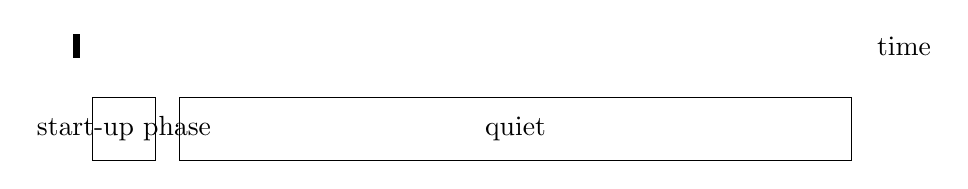
\begin{tikzpicture}[
    tick/.style={fill, inner sep=0pt, outer sep=0pt, minimum width=0.9mm,
      minimum height=3mm}]
  \node[tick] (t0) {};
  \node[right=100mm of t0] (tend) {time};
  \coordinate (b1) at ($(t0)!0.02!(tend.west)$);
  \coordinate (b2) at ($(t0)!0.10!(tend.west)$);
  \coordinate (b3) at ($(t0)!0.13!(tend.west)$);
  \coordinate (b4) at ($(t0)!0.98!(tend.west)$);
  \coordinate[below=9mm of t0] (band);
  \begin{scope}[on background layer]
    \node[draw, inner xsep=0pt, inner ysep=4mm, fit=(b1 |- band)(b2 |- band)] (busy) {};
    \node[draw, inner xsep=0pt, inner ysep=4mm, fit=(b3 |- band)(b4 |- band)] (quiet) {};
  \end{scope}
  \node (busy-t) at (busy.center) {start-up phase};
  \node (quiet-t) at (quiet.center) {quiet};
\end{tikzpicture}%
